% 2007 年湖南卷文科第 18 题：直二面角 α-PQ-β，A∈PQ，B∈α，C∈β。
% 来源 PDF：普通高考/2007/2007湖南文.pdf，SHA256 8e889ae321ffa864b24c505b40e7e96956b301487f5a106264b7fcd9f943e068
% 原页：第 2 页（A3 三栏）第 1 栏上部，印刷页 382，图在题干下方。
% 重绘依据：β 画成上半平面（竖直矩形），α 画成下半平面（平行四边形），交线 PQ 水平；
%   P 在左端、A 在 P 右侧、Q 在 A 右侧；C 在 β 内、B 在 α 内；
%   线段 CA、CB、AB 实线，平面轮廓与交线细实线，标注按原图。
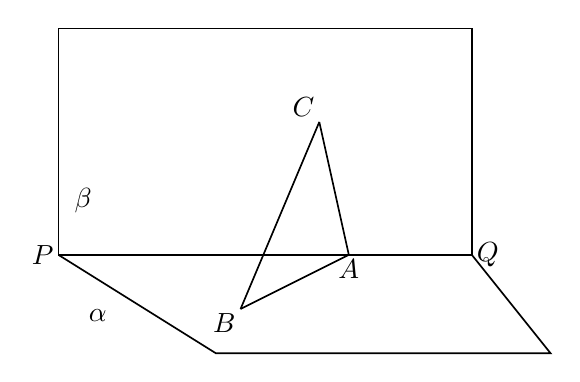
\begin{tikzpicture}[scale=1.25, semithick, every node/.style={inner sep=1.5pt}]
  % 平面 β（上）与 α（下）
  \draw (-2.6,0) -- (1.6,0) -- (1.6,2.3) -- (-2.6,2.3) -- cycle;
  \draw (-2.6,0) -- (-1.0,-1.0) -- (2.4,-1.0) -- (1.6,0);
  % 交线 PQ
  \draw (-2.6,0) -- (1.6,0);
  % 点
  \coordinate (P) at (-2.6,0);
  \coordinate (A) at (0.35,0);
  \coordinate (Q) at (1.6,0);
  \coordinate (C) at (0.05,1.35);
  \coordinate (B) at (-0.75,-0.55);
  % 关键线段
  \draw (C) -- (A);
  \draw (C) -- (B);
  \draw (A) -- (B);
  % 标注
  \node[anchor=east]  at (P) {$P$};
  \node[anchor=north] at (A) {$A$};
  \node[anchor=west]  at (Q) {$Q$};
  \node[anchor=south east] at (C) {$C$};
  \node[anchor=north east] at (B) {$B$};
  \node at (-2.35,0.55) {$\beta$};
  \node at (-2.2,-0.62) {$\alpha$};
\end{tikzpicture}
